\section{Graphical Design}

Based on our analysis, it turns out that there does not seem to be a relation between the complexity of the graphics, and the impact this has on how 
much fun, the game is or how educating the game is. For this reason 2D graphics has been deemed sufficient for this game. The following section will go 
through the design choices that has been made in terms of the graphical interface of the game, along with justification for why a given choice was made.

\subsection{World Map}

The world map is a hexagon consisting of smaller 'cells' which are also hexagonal. This means that by design the entire field is hexagons in hexagons. 
A cell takes up a single small-hexagon on the field, and as does the various food types a player may encounter.


\begin{figure}[h]
	\centering
		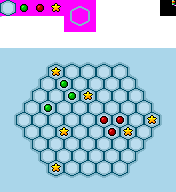
\includegraphics{img/cells_mockup.png}
	\caption{Playing field with cells and food}
	\label{fig:cells_mockup}
\end{figure}

As can be seen by the graphics, food in this example is a star. We have created other mock-ups as well, such as a typical cartoonish ham and an egg. 
Cells are illustrated on the map as green and red 'balls', with green refering to a specific player, and red refering to another player's cells. This 
sort of green and red distinction between the players will be used all throughout the game.


\subsection{Health Bar}

To give the players, when they compete, a way of getting an idea of how well they are doing in the game, we have decided to design a healthbar at the 
very top of the screen. The idea is that the healthbar will fill with green and red colors, depending on how well the game is going for one of the 
players.